\documentclass[11pt]{article}
\topmargin=0.0in %length of margin at the top of the page (1 inch added by default)
\oddsidemargin=0.0in %length of margin on sides for odd pages
\evensidemargin=0in %length of margin on sides for even pages
\textwidth=6.5in %How wide you want your text to be
\marginparwidth=0.5in
\headheight=0pt %1in margins at top and bottom (1 inch is added to this value by default)
\headsep=0pt %Increase to increase white space in between headers and the top of the page
\textheight=9.1in %How tall the text body is allowed to be on each page

\usepackage{url}
\usepackage{graphicx}
\usepackage{authblk}
\usepackage{wrapfig} % added from executive summary
\usepackage{etaremune}
\usepackage{hyperref}
\usepackage{amsthm}
\usepackage{amsmath}
\usepackage{listings} 
% \usepackage{draftwatermark}
% \SetWatermarkText{DRAFT}
% \SetWatermarkScale{5}
% "define" Scala
\lstdefinelanguage{scala}{morekeywords={class,object,trait,extends,with,new,if,while,for,def,val,var,this},
otherkeywords={->,=>},
sensitive=true,
morecomment=[l]{//},
morecomment=[s]{/*}{*/},
morestring=[b]"}
% Default settings for code listings
\lstset{frame=tb,language=scala,aboveskip=3mm,belowskip=3mm,showstringspaces=false,columns=flexible,basicstyle={\small\ttfamily}}

\renewcommand\Authfont{\fontsize{12}{14.4}\selectfont}
\renewcommand\Affilfont{\fontsize{9}{10.8}\selectfont}

\theoremstyle{plain}

\widowpenalty=500
\clubpenalty=500
\setlength{\parskip}{3pt}

\date{}

\begin{document}

\title{Parallel \emph{de novo} Assembly of Long Reads with \texttt{Ananas}}
\author{Frank~Austin~Nothaft}
\maketitle

\begin{abstract}
Genome assembly is a critical and expensive computational biology problem. The computational cost
of the problem is exacerbated by the difficulty of parallelizing the algorithm. In this paper,
we look at the overlap-layout-concensus formulation of the genome assembly problem. We introduce
the tool \texttt{Ananas}, which demonstrates linear scalability on a small dataset. \texttt{Ananas}
is built on top of the \texttt{ADAM} genomics API, using Apache \texttt{Spark} and \texttt{GraphX},
and parallelizes all stages of the algorithm.
\end{abstract}

\section{Introduction}
\label{sec:introduction}

One of the canonical computational biology problems is the genome assembly problem. In the
\emph{de novo} genome assembly problem, the goal is to sequence ``reads'' from the currently
unknown genome of an organism, and to ``assemble'' these fragments into long contiguous strings
(contigs) that best represent the underlying genome of the organism~\cite{pevzner01}.
There are two canonical graph-based formulations of this problem: we can either use a
\emph{de Bruijn}~\cite{pevzner01} or an \emph{overlap} graph~\cite{myers95} to reconstruct
genomic sequences.

In this paper, we look at parallelizing an overlap graph based assembler. We have chosen the
overlap graph approach, because although the \emph{de Bruijn} graph based approach is lower cost,
overlap graphs are better at resolving the repeat structure of genomes. This is caused by
\emph{de Bruijn} graphs collapsing down repeats that are larger than the $k$-mer size used
when creating the graph\footnote{$k$-mers are the $k$-letter length substrings that are used as
the vertices in a \emph{de Bruijn graph.}}. Additionally, we are interested in investigating
data generated with new sequencing technologies, such as Pacific Biosciences' Single Molecule
Real Time sequencing technology~(SMRT, \cite{eid09}) or the Oxford Nanopore technology~\cite{clarke09}.
These sequencing technologies generate very long reads\footnote{These technologies generate reads
with length in excess of $>10$ kilobase pairs (kbp). The most common sequencing vendor (Illumina)
generates reads with length typically less than $\sim250$bp.}---these long reads are easier to
use for generating high quality overlaps, and have lower asymptotic overlapping cost.

In an overlap graph based assembler, the assembly process can be broken up into three stages,
which is known as the OLC process:

\begin{enumerate}
\item First, we find the \textbf{overlaps} between all reads.
\item Then, we \textbf{layout} these reads as a graph, and simplify the graph.
\item Finally, we find the \textbf{concensus} sequence that this graph describes.
\end{enumerate}

In the remainder of this paper, we introduce \texttt{Ananas}, a parallel/distributed tool that
implements the OLC process. \texttt{Ananas} is implemented on top of \texttt{ADAM}~\cite{massie13,
nothaft15}, an Apache \texttt{Spark}-based~\cite{zaharia12, zaharia10} API for processing genomic
data. We implement a MinHash signature based method for computing read overlaps~\cite{berlin14},
which is parallelized using \texttt{Spark}. We then used the Apache \texttt{GraphX}~\cite{gonzalez14,
xin13} to build an overlap graph from the read overlaps. We reduced the overlap graph into a
string graph~\cite{myers05} and walked this graph to emit contigs. Our approach is fully parallel
and scales linearly out to four machines on a modest (1.5GB) input dataset. \texttt{Ananas} is
released as open source software under the Apache 2 license and is available from
\url{https://www.github.com/fnothaft/ananas}.

\section{Methods}
\label{sec:methods}

Although the read overlapping methods are close to embarassingly parallel, the graph traversal
methods are not as obviously data parallel. In this section, we will discuss our implementations
of both methods.

\subsection{Parallel Read Overlapping}
\label{sec:overlapping}

When computing the pairwise overlaps of reads, we are trying to identify reads that are highly
similar. Although traditional overlapping algorithms tend to be index-based~\cite{myers14}, we
use a MinHash signature based method which was originally proposed by Berlin et al~\cite{berlin14}.
While a na\"{i}ve overlapper will attempt to compute the full $\mathcal{O}(n^2)$ pairwise overlaps,
a locality sensitive hashing~(LSH) scheme can be used to reduce the number of overlaps computed to
$\mathcal{O}(\frac{n^2}{b})$, where $n$ is the number of reads in the dataset and $b$ is the number of
buckets used for the LSH~\cite{leskovec14}. Additionally, using MinHash signatures allows us to
decrease the cost of approximately comparing two sequences. Comparing two MinHash signatures has
time complexity $\mathcal{O}(s)$, where $s$ is the signature length, while the time complexity of
local sequence alignment is $\mathcal{O}(n_1 n_2)$, where $n_1, n_2$ are the lengths of the two
sequences being compared~\cite{smith81}.

MinHash signatures are useful as they can be used to rapidly compute approximate similarity
measures of two sequences. First, for two sets $S_1, S_2$, the Jaccard similarity of these
two sets is given by equation~\eqref{eqn:jaccard}. If the two sets yield length $s$ signatures
$S_1 \rightarrow M_1, S_2 \rightarrow M_2$, their similarity can be approximated by equation
\eqref{eqn:minhash-jaccard}.

\begin{align}
\label{eqn:jaccard}
\text{Jaccard Similarity} &= \frac{| S_1 \cap S_2 |}{| S_1 \cup S_2 |} \\
\label{eqn:minhash-jaccard}
\text{Jaccard Similarity} &\sim \frac{\sum_{i = 1}^s I^{[M_1^i = M_2^i]}}{s} 
\end{align}

The process for computing the signature of a read is straightforward. First, we generate
a length $s$ array $R$ of random integers, where $s$ is the signature length we are using.
Then, we ``shingle'' each element of our input dataset: shingling extracts length $n$ token
overlaps, where $n$ is a user provided parameter. The semantics of the shingles depends on
the input dataset: for traditional document similarity comparison, $n$-gram shingles are
typically used, where an $n$-gram is a sequence of $n$ consecutive words and where consecutive
$n$-grams have $n - 1$ words in common~\cite{leskovec14}. In our application, we use $k$-mers
and set $k = 16$, which allows us to bit pack each $k$-mer into a 32-bit integer\footnote{We
use \emph{canonical} $k$-mers. To generate a canonical $k$-mer, we take the lexicographically
first $k$-mer out of this $k$-mer and it's reverse complement $k$-mer. To generate the reverse
complement of a $k$-mer, we reverse the $k$-mer string and ``flip'' the bases in the string
using the \texttt{A} $\leftrightarrow$ \texttt{T}, \texttt{C} $\leftrightarrow$ \texttt{G}
mapping. As we will discuss later, this is critical as reads may be sequenced from either
strand of a DNA molecule.}. Once we have generated the shingles, we apply a hash function
to each shingle that maps $T \mapsto \text{Int}$, where $T$ is the type of the shingle. In
our case, we are bitpacking the $k$-mers into integers, and we are able to just emit the
integer value of the bitpacked canonical $k$-mer as our hash. Given the length $n_i - k + 1$
hash vector $H_i$ of read $i$ (where $n_i$ is the read length and $k = 16$ is the $k$-mer
shingle length) and the length $s$ array $R$ of random integers, we compute the signature
$M_i$ of read $i$ using equation~\eqref{eqn:minhash-signature}, where $\oplus$ is the
bitwise XOR of two integers.

\begin{align}
\label{eqn:minhash-signature}
M_i[j] = \min_{h \in H_i} h \oplus R[j], \forall j \in \{0, \dots, s - 1\}
\end{align}

To run this process, we start by converting each read sequence into an indexed \emph{de Bruijn}
sequence, which we have introduced in \cite{nothaft15thesis}\footnote{An indexed \emph{de Bruijn}
sequence is a list of $k$-mers which are tagged with the position where the $k$-mer occurred in
the graph. Since two adjacent $k$-mers in a sequence trivially satisfy the $k - 1$ base condition
necessary to place an edge in a \emph{de Bruijn} graph, this list is an equivalent representation
of a graph. While we solely use this structure to shingle reads for our hashing scheme, this
structure is highly applicable in the local sequence assembly case (see ch. 3 of our other
text~\cite{nothaft15thesis}, and we plan to make further use of the datastructure in a future
version of \texttt{Ananas}.}. This process is embarassingly parallel and is implemented by
\texttt{map}ping over an input Resilient Distributed Dataset~(RDD, see~\cite{zaharia12}).
Simultaneously, we generate an array of hashes for use in generating the MinHash signatures of
each sequence and broadcast this array of hashes to each node.

As noted above, once these signatures have been computed, we still need to compute all pairwise
alignments. While we do support computing the full cartesian overlap, we rely in practice on
the LSH scheme illustrated by Berlin et al~\cite{berlin14} and formalized by Leskovec et
al~\cite{leskovec14}. In this approach, we map each signature to $b$ buckets and only estimate
overlaps within these buckets. We require that $s \bmod b = 0$. The significance of this is
that $p = \frac{b}{s}$ hashes from the MinHash signature of read $R_i$ are used to determine
the buckets to send $R_i$ to. To implement this operation, we perform a \texttt{flatMap} over
all read signatures, and compute $b$ bucket IDs. The bucket IDs are tuples of integers and
length $p$ integer arrays. We compute the ID tuple $T_i^b$ for bucket $b$ from read $R_i$ with
signature $M_i$ using equation~\eqref{eqn:lsh}.

\begin{align}
\label{eqn:lsh}
T_i^b = (b, M_i[p b:p (b + 1) - 1])
\end{align}

Once we have \texttt{flatMap}ped all reads, we \texttt{groupBy} each key to collect an array
containing all reads that fall into each bucket. We then run a pairwise comparison of all
signatures inside of each bucket. It is worth noting that two reads can pairwise map into
multiple buckets (i.e., both $R_1$ and $R_2$ will map into bucket $(0, [h_0, h_1])$ and bucket
$(1, [h_2, h_3])$ if $M_1[0:3] = M_2[0:3]$). This can lead to us emitting duplicate overlaps.
To handle this, we only evaluate a pairwise overlap if this is the ``earliest'' bucket where
the two reads could have met. We impose an ordering by looking at the integer in the tuple; in
the example given earlier, we would only evaluate the overlap of the two reads in bucket $(0,
[h_0, h_1])$.

When we evaluate an overlap, we emit the approximate similarity score given by
equation~\eqref{eqn:minhash-jaccard}. We immediately filter all overlaps where the
estimated overlap length is below a user provided threshold (the estimated overlap $o_e$
is given by $s_{1,2} \max n_1, n_2$, where $s_{1,2}$ is the estimated similarity between
the two reads and $n_1, n_2$ are the lengths of the two reads). If the read pair passes the
similarity threshold, we then compute the exact overlap length. We do this by finding the
size of the intersection of the two indexed \emph{de Bruijn} sequences. Additionally, we
compute several other properties:

\begin{itemize}
\item Does this overlap switch strands? When we create the canonical $k$-mers in the \emph{de
Bruijn} sequence, we log whether the $k$-mers were originally canonical or not. If the
overlapping $k$-mers had different original canonicality, we note that the reads are sequenced
from different strands.
\item At what end of the read does the overlap start from? Does the overlap contain the
beginning or end of the read, or is the entire read overlapped by a longer read?
\end{itemize}

While the approach outlined in this section improves the runtime complexity of overlapping,
it comes at the cost of data being duplicated at a factor of $b$. In~\S\ref{sec:discussion},
we discuss a possible solution to this problem.

\subsection{Parallel Graph Simplification and Traversal}
\label{sec:graph-simplification-traversal}

Once we have emitted the overlaps, we use these overlaps to create a graph in
\texttt{GraphX}~\cite{gonzalez14, xin13}. From here, we run transitive reduction to simplify
the graph, and then walk the graph to emit contigs. The graph operations were complicated
because \texttt{GraphX} uses an underlying representation that assumes a directed graph.
In a two-strand sequencing process, overlap graphs are bidirected.

The transitive reduction algorithm for reducing an overlap graph into a string graph was
introduced by Myers~\cite{myers05}. Our goal is to remove all redundant edges while maintaining
all true paths by simplifying the graph. While transitive reduction is well defined for a
directed, acyclic graph\footnote{Specifically, at vertex $A$, with neighbors $\mathcal{N} =
B, \dots, Z$, we preserve reachability if we eliminate all edges from $A \rightarrow n, n \in
\mathcal{N}$ if there exists a walk $A \rightarrow o_1 \rightarrow \dots \rightarrow n$.}
its definition is unclear for a bidirected, possibly cyclic graph. While Myers~\cite{myers05}
effectively defines the transitive reduction of an overlap graph to be any graph that has not
oversimplified the presence of a sequence variant, we find this definition to be imprecise.
We define the following rules for transitively reducing an overlap graph:

\begin{itemize}
\item Disregard all reads that are fully overlapped by another read. They can trivially be
merged into the longest read that fully contains them.
\item Treat all other edges as undirected. If there is an admissible triangle containing
reads $A, B, C$, each node should greedily pick to keep the edge with the longest overlap
length at it's start and end. E.g., if $A$---$B$ has overlap of 500 bp, $B$---$C$ has overlap
of 500 bp, and $A$---$C$ has overlap of 300 bp, we will choose to keep $A$---$B$---$C$ and
will eliminate $A$---$C$.
\end{itemize}

Note in the rules above that we only process \emph{admissible} triangles. Specifically,
we only process triangles where all read alignments are concordant. Temporarily assuming
a single stranded sequencing protocol, a triangle $\triangle ABC$ would be admissible if the
$A$---$B$ overlap began at the end of $A$ and the start of $B$, the $B$---$C$ overlap
begin at the end of $B$ and the start of $C$, and the $A$---$C$ overlap began at the
end of $A$ and the start of $C$. Additionally, if the $A$---$B$ overlap is longer than
the $A$---$C$ overlap, the $B$---$C$ overlap must also be longer than the $A$---$C$
overlap. In our implementation, we keep any edges where a single node votes to keep the
edge. Given the restrictions on admissibility above, this is provably correct. In this
proof, we assume a single stranded sequencing protocol for simplicity. A directed edge
from $A \rightarrow B$ implies that there is an overlap from the end of $A$ to the
beginning of $B$.

\begin{proof}
First, consider the case where the triangle is inadmissible:

\begin{itemize}
\item If the triangle is inadmissible because the overlap directions are not concordant,
this implies that the triangle describes a loop in the graph. Specifically, $A \rightarrow
B$, $B \rightarrow C$, $C \rightarrow A$ implies that there is an inversion of the sequence
contained in read $A$. This loop cannot be reduced, but vertices $B, C$ can be merged.
\item If the triangle is inadmissible because of the lengths of the overlaps are discordant,
this implies that the triangle describes a large allelic divergence, such as an insertion/deletion
variant. Since this triangle describes two sequence variants, it cannot be reduced nor can
any vertices be merged.
\end{itemize}

In the case that the triangle is admissible, $A, B,$ and $C$ will all vote for the same edges.
A proof of this is trivial. However, for this proof to be valid, our approach must satisfy a
graph with multiple triangles. This is true. Observe a graph $A$---$B$---$C$---$D$---$E$,
$A$---$C$---$E$, $B$---$D$. If the simplest reducible graph is $A$---$B$---$C$---$D$---$E$,
triangles $\triangle ABC$, $\triangle BCD$, and $\triangle CED$ will all be admissible and will
vote for $A$---$B$---$C$---$D$---$E$.
\end{proof}

While this problem statement is straightforward, it is somewhat difficult to map to the
vertex-centric \texttt{GraphX} API. To implement this algorithm, each vertex collects its
edge attributes, which is then joined against the graph. We then run an iteration of message
passing where each vertex sends its edges to all neighbor vertices. At this point,
each vertex knows what edges it has, and what edges each neighbor has. We then separate the
neighbor edges into overlaps that start at the start/end of the read, and run a tail-recursive
algorithm that implements the triangle voting process. Once each node has run its voting
process, we run a subgraph operation. This subgraph operation is used to keep only edges
who were voted for. No nodes are dropped from the graph.

Once we have run transitive reduction on the graph, we emit contigs. While conceptually we
could merge all edges that have unit in/out degree into a larger node and then estimate
node copy number~\cite{myers05}, we decided not to implement these features for two reasons:

\begin{itemize}
\item Merging edges together is only necessary for estimating node copy number, and is difficult
to implement in the \texttt{GraphX} API, which assumes that graphs are immutable (with the
exception of allowing subgraphs to be created).
\item The formulation of node copy number presented by Myers~\cite{myers05} requires the
development of a \texttt{GraphX}-based solver for min cost flow, which was intractible given the
project timelines.
\end{itemize}

To generate contigs, we ran a graph labeling algorithm that is similar to \texttt{GraphX}'s
implementation of connected components labeling. We started by collecting all edges to each
vertex, and sorting these edges into start/end vertices. From here, we ran the following
algorithm:

\begin{enumerate}
\item If a node has either no start or no end vertices, it chooses to send a message in
the initial iteration. This message contains the node ID. This ID is used to label the
generated contig.
\item At each iteration, if a node has received a message, it logs the ID of the node
that started the message passing in the initial iteration, and the ID of the node that
message came from. If the node that is sending a message has any edges on the side
\emph{opposite} from where the message came from (e.g., if the message came in from the
start of the read, it needs to go out on an edge from the end of the read), we send a
message on that edge in the next round.
\end{enumerate}

This algorithm is implemented using \texttt{GraphX}'s \texttt{Pregel} abstraction~\cite{malewicz10}
and runs until no more messages can be sent. There are several important implementation
details:

\begin{itemize}
\item If our graph contains a single connected component where all but two edges have in/out degree
of one, we will send two messages in the inital iteration. These two messages will describe
the same contig. To handle this, when the two messages reach the same node, we pick the message
with the lowest starting node ID and relabel all nodes tagged with the previous starting node
ID. This is why we store both the starting node ID and the message sender ID.
\item In \texttt{GraphX}'s implementation of \texttt{Pregel}, node updates can only occur on update.
This implies that vertex state cannot be mutated when sending messages. To ensure that a node does
not send multiple messages to the same vertex, we choose the message recipients for the next
iteration when we are processing the received messages. Additionally, we track an iteration
count with each message. Since \texttt{GraphX} only activates vertices that received a message in
the last iteration, we are able to track what messages to send by looking for the labels that
have the highest iteration count.
\end{itemize}

Once we have run this algorithm, we \texttt{flatMap} each vertex sequence and key by the starting
node ID. We also track the strandedness relative to the starting node, and the iteration in which
the node was tagged. We then \texttt{groupBy} the key (the starting node ID), sort all subsequences,
and reverse complement sequences as necessary. Finally, we use \texttt{ADAM}~\cite{massie13, nothaft15}
to save all contigs from \texttt{Spark} in a parallel manner.

\section{Results}
\label{sec:results}

We evaluated \texttt{Ananas} on Amazon's Elastic Compute 2 (EC2) cloud, using the \texttt{r3.2xlarge}
instance type. We evaluated \texttt{Ananas} on PacBio~\cite{eid09} sequence of the \texttt{E. coli}
virus\footnote{This sequence was captured using an RS II  with P6/C4 chemistry. The dataset is available
from \url{https://github.com/PacificBiosciences/DevNet/wiki/E.-coli-20kb-Size-Selected-Library-with-P6-C4}
and was preprocessed with \texttt{SMRT$^\copyright$ Analysis} to convert to FASTA format.}. We evaluated
on two and four nodes, and saw linear speedup between these two nodes. This can be seen in
Figure~\ref{fig:speedup}.

\begin{figure}[h]
\begin{center}
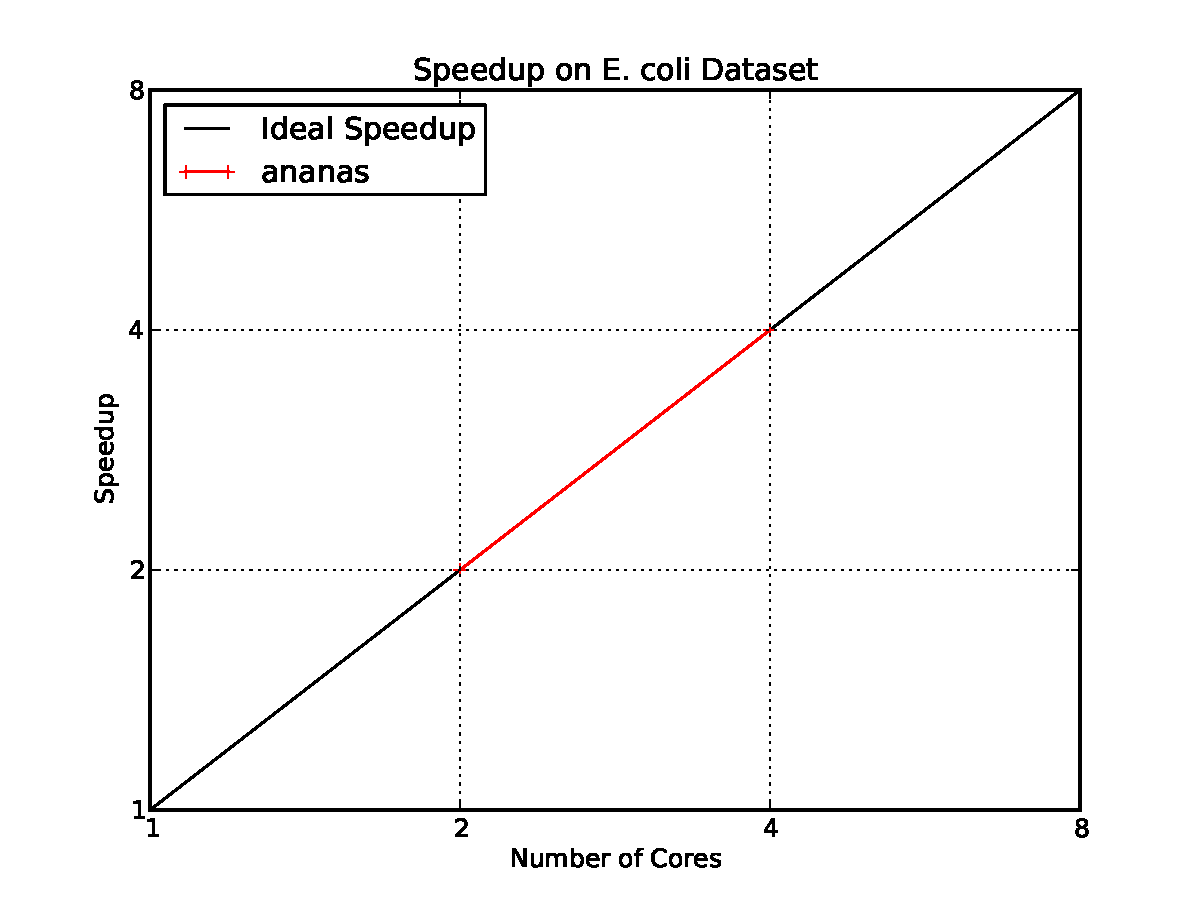
\includegraphics[width=0.4\linewidth]{graphs/speedup.pdf}
\end{center}
\caption{Speedup across nodes}
\label{fig:speedup}
\end{figure}

For our speedup experiments, we used an overlap cutoff of 500 bp and 4 buckets. With this configuration,
approximately 10\% of time was spent on overlapping, 70\% was spent on transitive reduction, and
20\% was spent on contig generation. Although the speedup is linear, the performance is poor. On four
machines, it took approximately 50 minutes to process the \emph{E. coli} dataset, which is worse than
expected. However, it is worth noting that while this number is worse than hoped, 50 minutes on four
eight core machines represents approximately 27 core hours, which is approximately $5\times$ better
than the performance of the error correction step for a hybrid PacBio assembly system on \emph{E. coli}
data~\cite{koren12}. In future work, we plan to perform a more thorough evaluation against prior tools.

\begin{figure}[h]
\begin{center}
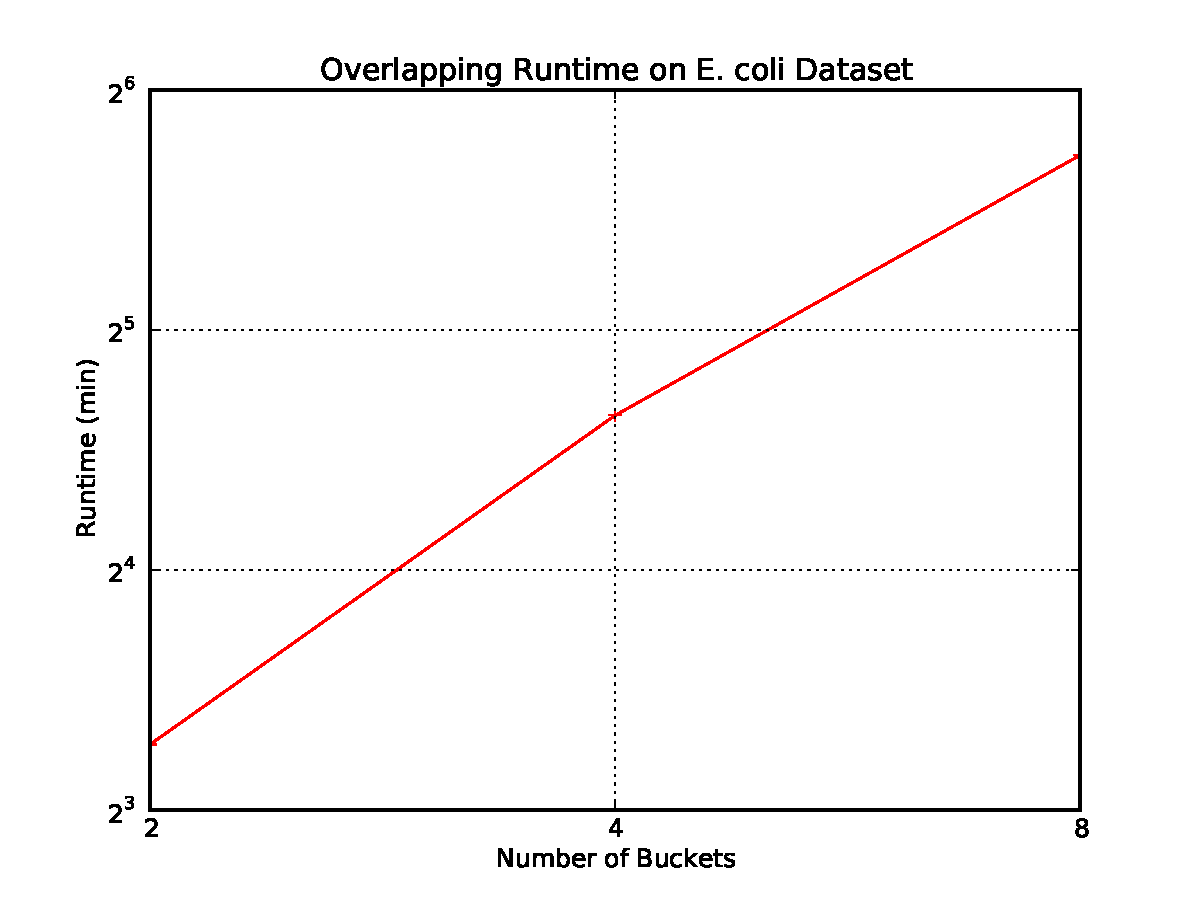
\includegraphics[width=0.4\linewidth]{graphs/overlap.pdf}
\end{center}
\caption{Overlapping performance vs. bucket size}
\label{fig:overlap}
\end{figure}

Overlapping performance should scale with the number of buckets in use. Specifically, a two-fold increase
in the number of buckets we evaluate leads to a two-fold increase in data (due to replication during the
\texttt{flatMap}) and a two-fold increase in the number of comparisons performed. To evaluate this, we
swept the number of buckets used during overlapping from two to four to eight and performed overlapping
on two machines. This is shown in Figure~\ref{fig:overlap}. This trend held close to true; while the
increase in runtime was slightly greater than two going between two and four buckets, it was slightly
less than two when going from four to eight buckets.

\section{Discussion}
\label{sec:discussion}

We will continue to improve \texttt{Ananas} after this project has completed. We are interested in
improving performance via better overlapping schemes, and by improving the cost of transitive
reduction. Additionally, we would like to move to a better scheme for generating contigs.

As explained in~\S\ref{sec:overlapping}, our overlapping performance is impacted by the bucket count,
$b$, used for overlapping. One approach that can be used to further improve overlapping performance
is to move to a multi-probe LSH approach~\cite{lv07}. In this scheme, a likelihood function is used
to predict the buckets to materialize. This allows us to eliminate ``unproductive'' buckets, which
leads to a reduction in the number of reads duplicated and the number of comparisons performed.

Currently, our runtime is dominated by the transitive reduction phase. We are looking into ways to
improve the performance of this phase. Specifically, we think there may be ways to recast the
implementation. Although the algorithm we introduce in~\S\ref{sec:graph-simplification-traversal}
is cast as a triangle-based algorithm, due to the APIs provided by \texttt{GraphX}, we implement
the algorithm by materializing edges to vertices. We may be able to improve performance by modifying
the \texttt{GraphX} core.

Finally, we would like \texttt{Ananas} to support variable ploidy assembly. While \texttt{Ananas}
currently assembles contigs assuming that the underlying organism is haploid (there is a single
copy of each chromosome, and thus a single path through the graph), this assumption is unrealistic
for many organisms~\cite{paten14}. To do this, we would like to call the \emph{copy number} of each
segment: Myers~\cite{myers05} describes a min cost flow based approach for calling the number of paths
through each node by reweighting the edges. Although the approach presented by Myers can be efficiently
implemented, it is not clearly justified from a theoretical perspective. We propose using a likelihood
based formulation for calling edge multiplicity (and thus vertex copy number from in/out degree).
An approach similar to \texttt{CGAL}~\cite{rahman13} could be used; \texttt{CGAL} itself cannot be
used as it assumes a mate pair\footnote{In many ``short read'' sequencing techniques, sequencing
libraries are constructed with read pairs. In this paradigm, two reads are generated from a single
DNA sequence.} structure that is not applicable to long read datasets.

\section{Conclusion}
\label{sec:conclusion}

In this paper, we have introduced \texttt{Ananas}, a parallel/distributed \emph{de novo} assembler
for long read genomic data. \texttt{Ananas} is built on top of \texttt{ADAM}~\cite{massie13,
nothaft15}, Apache \texttt{Spark}~\cite{zaharia12, zaharia10}, and \texttt{GraphX}~\cite{gonzalez14,
xin13}. We have evaluated \texttt{Ananas} on \emph{E. coli} data and found that it scales linearly across
four machines. Additionally, we have demonstrated a parallel way to implement approximate MinHash-based
overlapping, and have provided a formalized algorithm for transitive reduction over overlap graphs.
This algorithm can be probably parallelized across all triangles in a graph.

\bibliographystyle{abbrv}
\bibliography{ananas}

\end{document}
